\section{System Overview}
\label{sec:System_Overview}
The aggregate system is shown in Figure \ref{fig:sys_overview} and consists of a manipulator, a gripper, an object, a tracking system, control computers, a fluidic drive array and a rigid frame.
The planar six segment soft rubber manipulator consists of twelve distributed elastomer actuators. This manipulator moves with minimal friction on a level plane.
A soft rubber gripper is fixed to the tip of the manipulator.
An object is randomly placed within the reachable envelop of the manipulator. 
A motion capture system provides real-time measurements of marked points both along the inextensible back of the manipulator and on top of the object. 
\rkk{We used the motion capture system OptiTrack Flex 3 by by Natural Point, Inc.}
The grasp motion planning algorithm as well as the curvature controller run on the control computers and take the tracking information as input.
The curvature controller then provides continuous closed-loop adjustment of the fluidic drive cylinder array.
The cylinder array directly actuates the manipulator and gripper.
A rigid frame holds all the subsystems together providing reliable and consistent hardware experiments. 
\rkk{The frame serves also as a mobile presentation platform that keeps the complete system together and holds the tracking cameras rigidly in place, not requiring recalibration after moving the system around.}

\begin{figure}[htbp]
\begin{centering}
  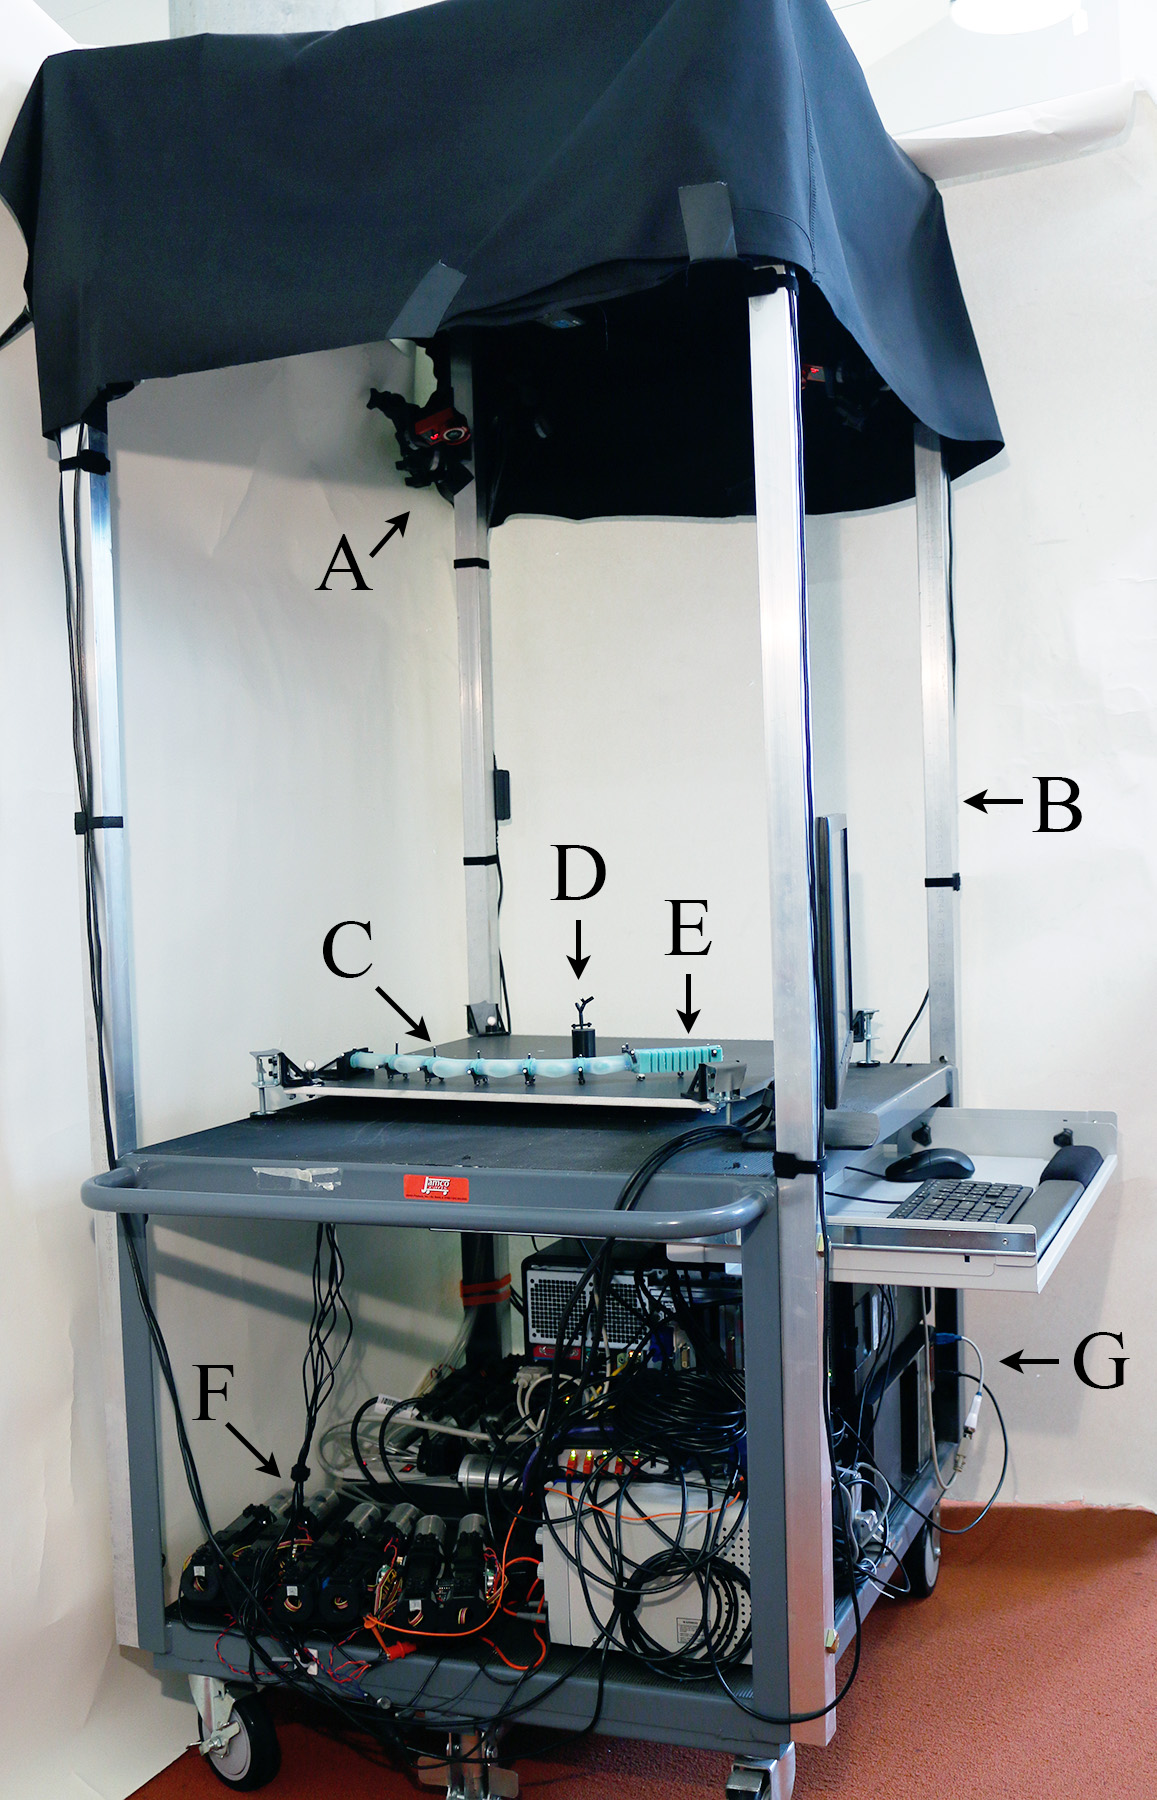
\includegraphics[width=2.0in]{Figures/system_overview/sys_overview_smaller}\\
  \caption{System Overview. The system is composed of (\textbf{A}) a motion capture system, (\textbf{B}) rigid frame, (\textbf{C}) soft six segment planar manipulator, (\textbf{D}) an object within the grasp envelope, (\textbf{E}) a soft gripper fixed to the manipulator, (\textbf{F}) a fluidic drive cylinder array to control actuation, and (\textbf{F}) computers for real-time processing and control.} \label{fig:sys_overview}
\end{centering}
\end{figure}
